\subsection{Gleichstrommaschine}

Die Steuerung wird mit  einer Gleichstrommaschine Realisiert. Daf\"ur wird das
Ersatzschaltbild   in   der  Abbildung  \ref{fig:dc-motor-ersatz}   verwendet.

\begin{figure}[H]
    \centering
    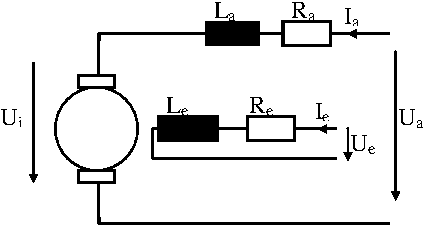
\includegraphics[width=\imagewidth]{images/dc_motor_ersatz}
    \caption{Ersatzschaltung der Gleichstrommaschine. Die eingezeichneten Strom- und Spannungsrichtungen entsprechen dem Verbrauchersystem.}
    \label{fig:dc-motor-ersatz}
\end{figure}

Die relevanten Gleichungen f\"ur die elektrische Dom\"ane sind:

\begin{align}
    U_a &= R_a \cdot i_a + L_a \cdot \frac{di_a}{dt} + U_i \\
    U_e &= R_e \cdot i_e + L_e \cdot \frac{di_e}{dt}
\end{align}

In der Mechanischen Dom\"ane:

\begin{equation}
    M_{el} = M_{Welle} + M_R + J\frac{d\omega_m}{dt}
\end{equation}

Die  elektrische  und  mechanische  Dom\"anen sind nach dem  folgenden  Gesetz
gekoppelt:

\begin{align}
    U_i    &= c\phi\omega_m \\
    M_{el} &= c\phi I_a
\end{align}

Die   Gleichstrommaschine   kann  in  verschiedene  Arten  geschalten   werden
(Fremderregt, Nebenschluss und Hauptschluss). Wir verwenden  die  fremderregte
Schaltungsart,  aus dem Grund, weil so die Drehzahl  \textit{linear}  mit  der
Belastung   abnimmt   und  alles  was  sich  linear  verh\"alt  ist   in   der
Regelungstechnik bevorzugt und einfacher zu steuern.

F\"ur diese  Schaltungsart  wird  der Erregerkreis unabh\"angig vom Ankerkreis
gespeist. So  kann  der  Erregerfluss  unabh\"angig vom Ankerstrom eingestellt
werden. Es gilt:

\begin{equation}
    U_a = U_i + R_aI_a = c\phi_e\omega_m + R_aI_a
\end{equation}

$\phi_e$ bleibt konstant sofern $I_e$ auch konstant bleibt.


